Para comparar o impacto da performance de diferentes tipos de cruzamentos na função $f6$,
foram obtidos os resultados apresentados na tabela \ref{tab:f6_crux} utilizando, cruzamento de um ponto,
de dois pontos, de 10 pontos e cruzamento uniforme. A representação, seleção, operadores genéticos
e critério de paragem utilizando foram os mesmos utilizados na seção 1.

\begin{table}[htb]
	\centering
	\begin{tabular}{|c|c|c|}
		\hline
		\rowcolor[HTML]{9B9B9B}
		Cruzamento & Média melhor indíviduo & Média população \\\hline
		1 ponto & 0.94532 & 0.81428 \\\hline
		2 pontos & 0.96801 & 0.79992 \\\hline
		10 pontos & 0.98094 & 0.73474 \\\hline
		Uniforme & 0.96441 & 0.85488 \\\hline
	\end{tabular}
	\caption{Resultados da função $f6$ utilizando vários tipos de cruzamentos \label{tab:f6_crux}}
\end{table}



\begin{figure}[htb]
	\begin{subfigure}{.45\textwidth}
		\centering
		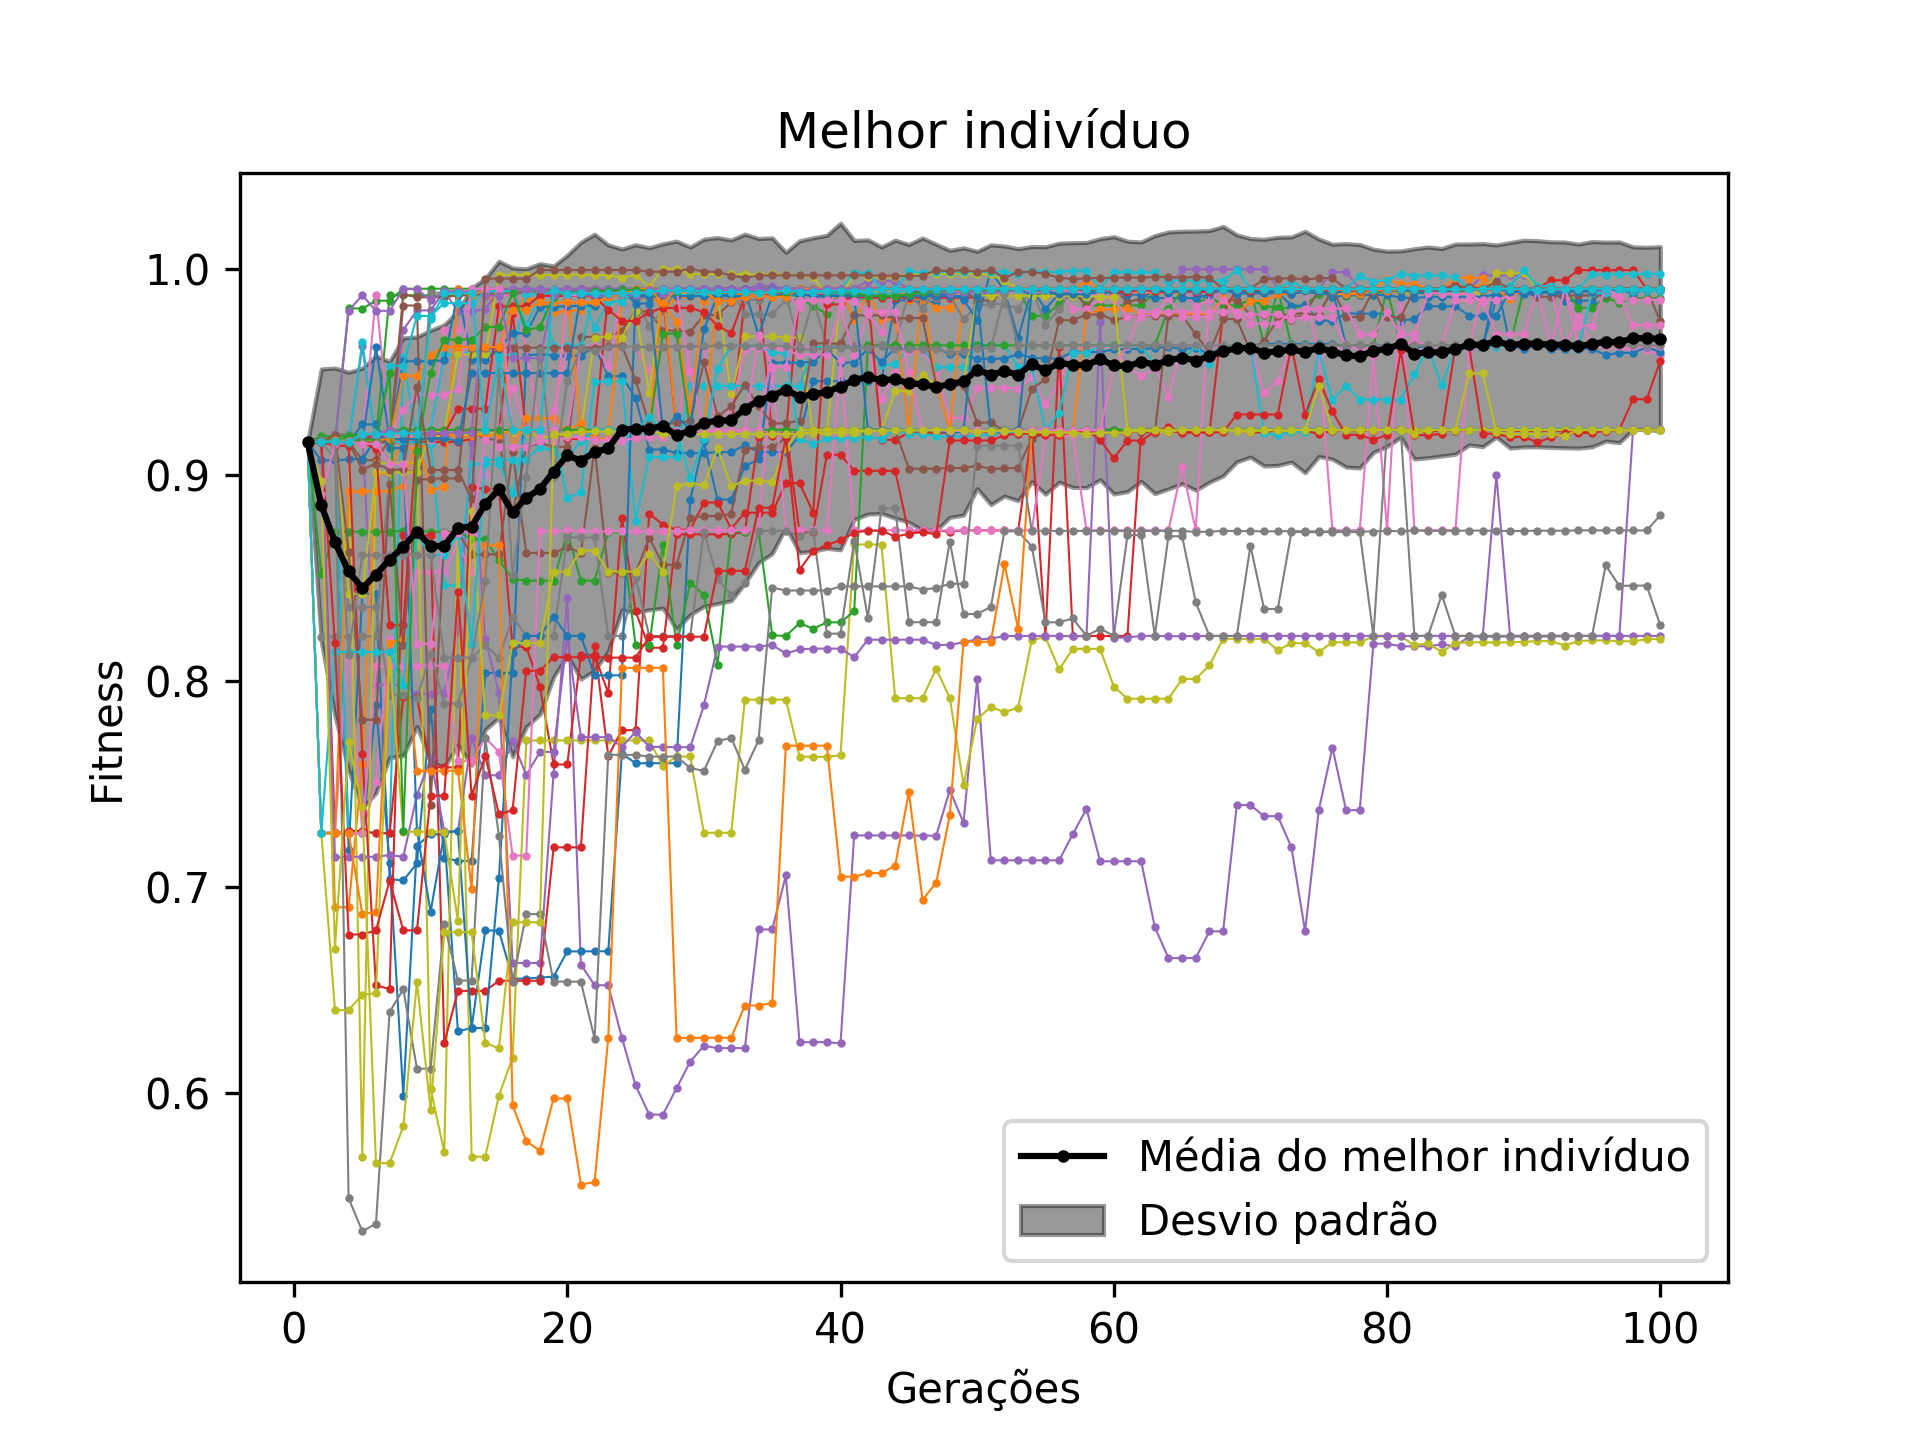
\includegraphics[width=1\textwidth]{sec-02/f6_1p_fitness_vs_gen_best.png}
		\caption{Melhores indíviduos de todos os experimentos ao longo das gerações.
		Em preto é mostrado o comportamento médio dos 50 experimentos. }
	\end{subfigure}
	\hfill
	\begin{subfigure}{.45\textwidth}
		\centering
		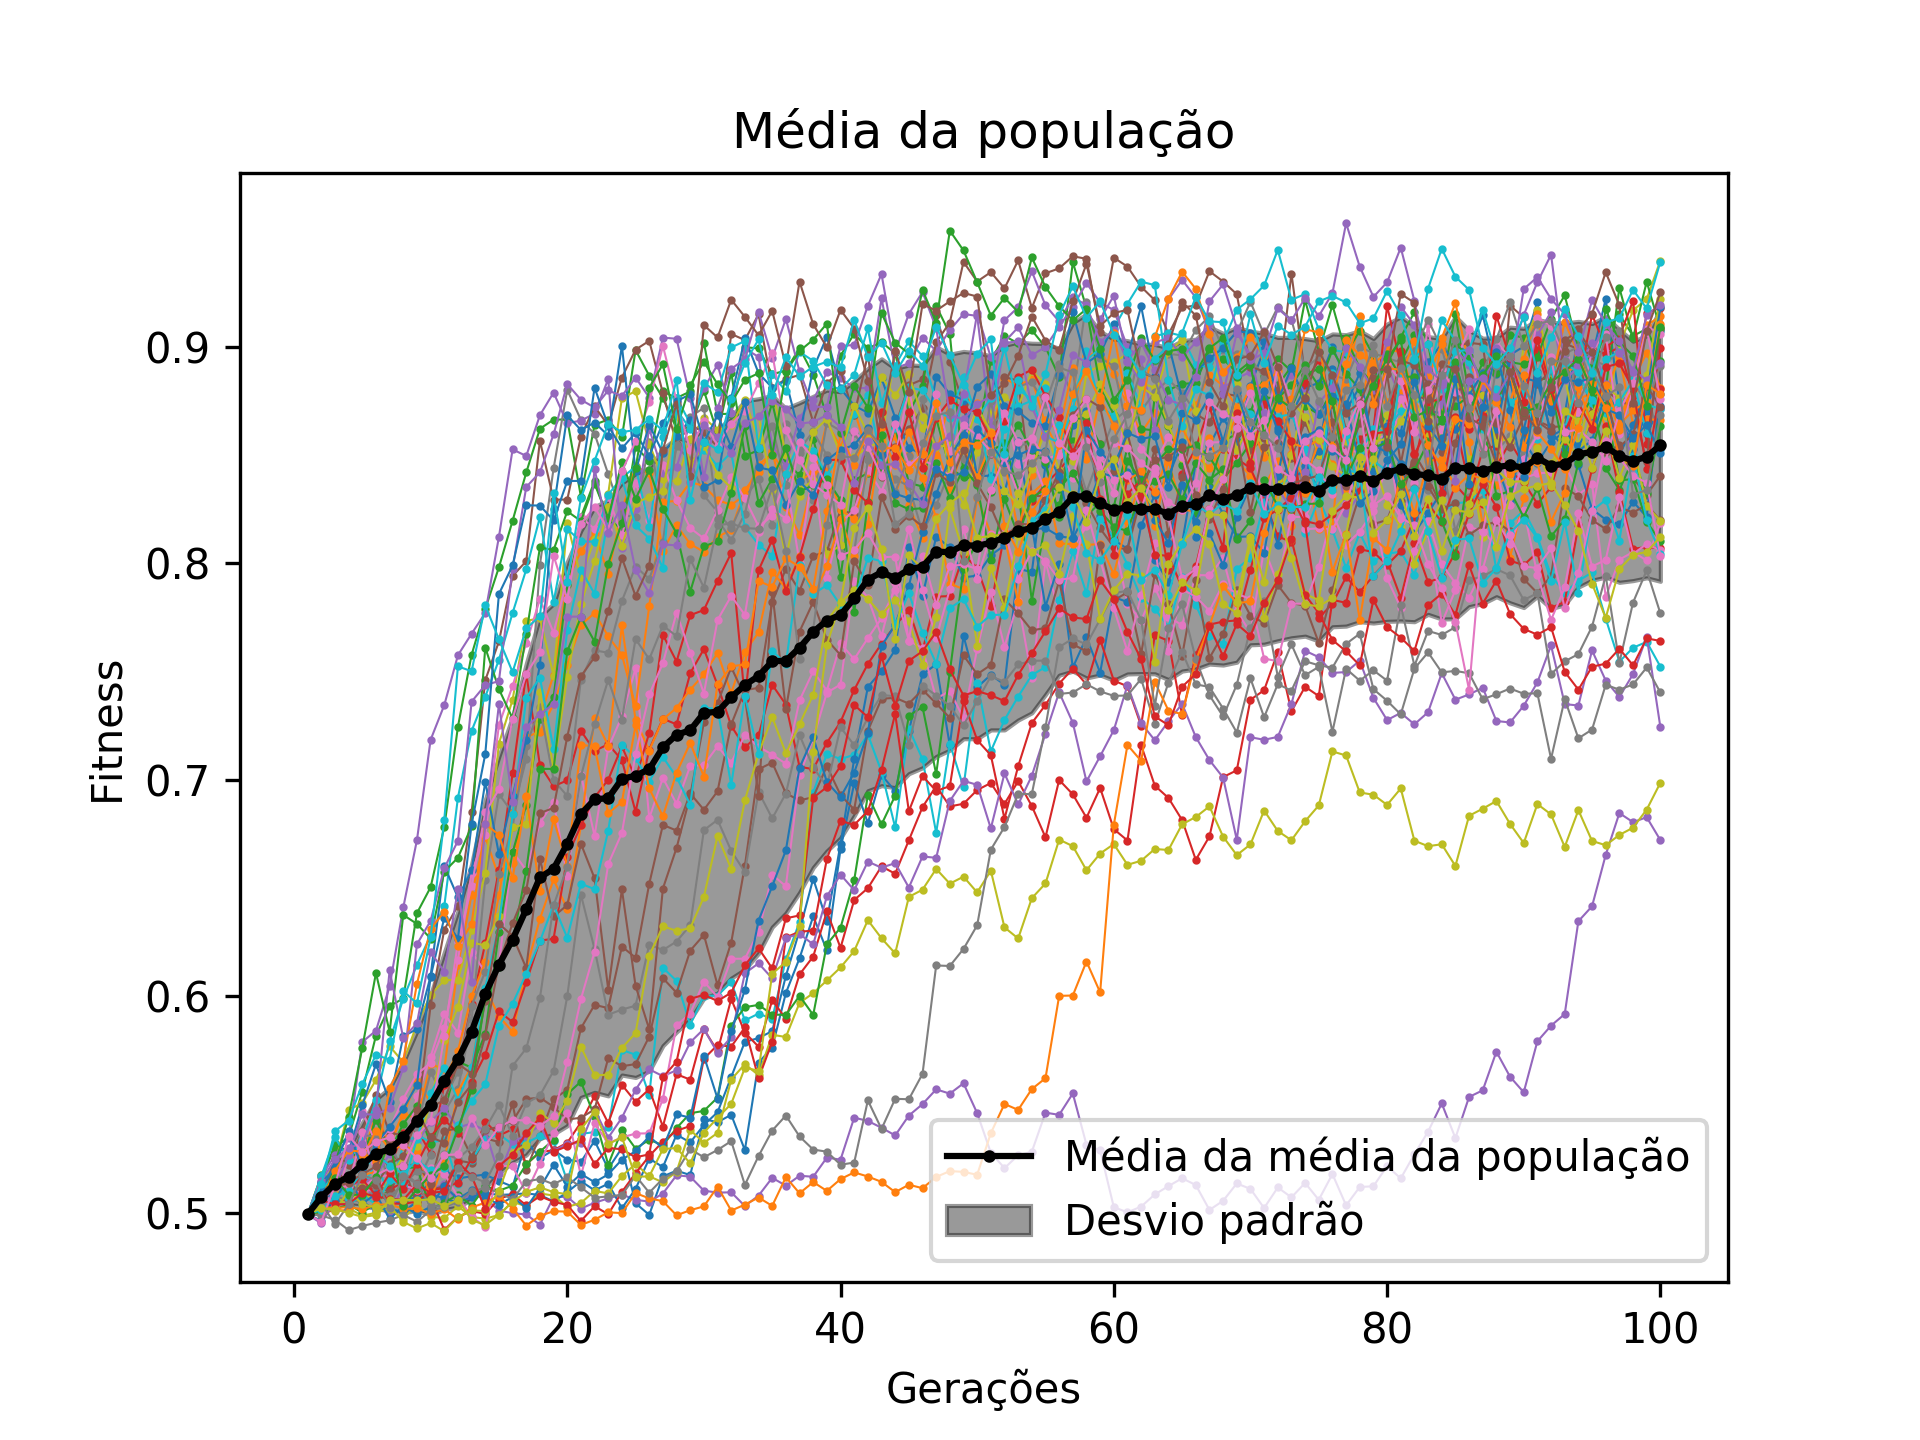
\includegraphics[width=1\textwidth]{sec-02/f6_1p_fitness_vs_gen_pop.png}
		\caption{Média da população de todos os experimentos ao longo das gerações.
		Em preto é mostrado o comportamento médio dos 50 experimentos.}
	\end{subfigure}
	\caption{Resultados obtidos para o caso de cruzamento de 1 ponto apresentado na tabela~\ref{tab:f6_crux}}
\end{figure}


	\begin{figure}[htb]
	\begin{subfigure}{.45\textwidth}
		\centering
		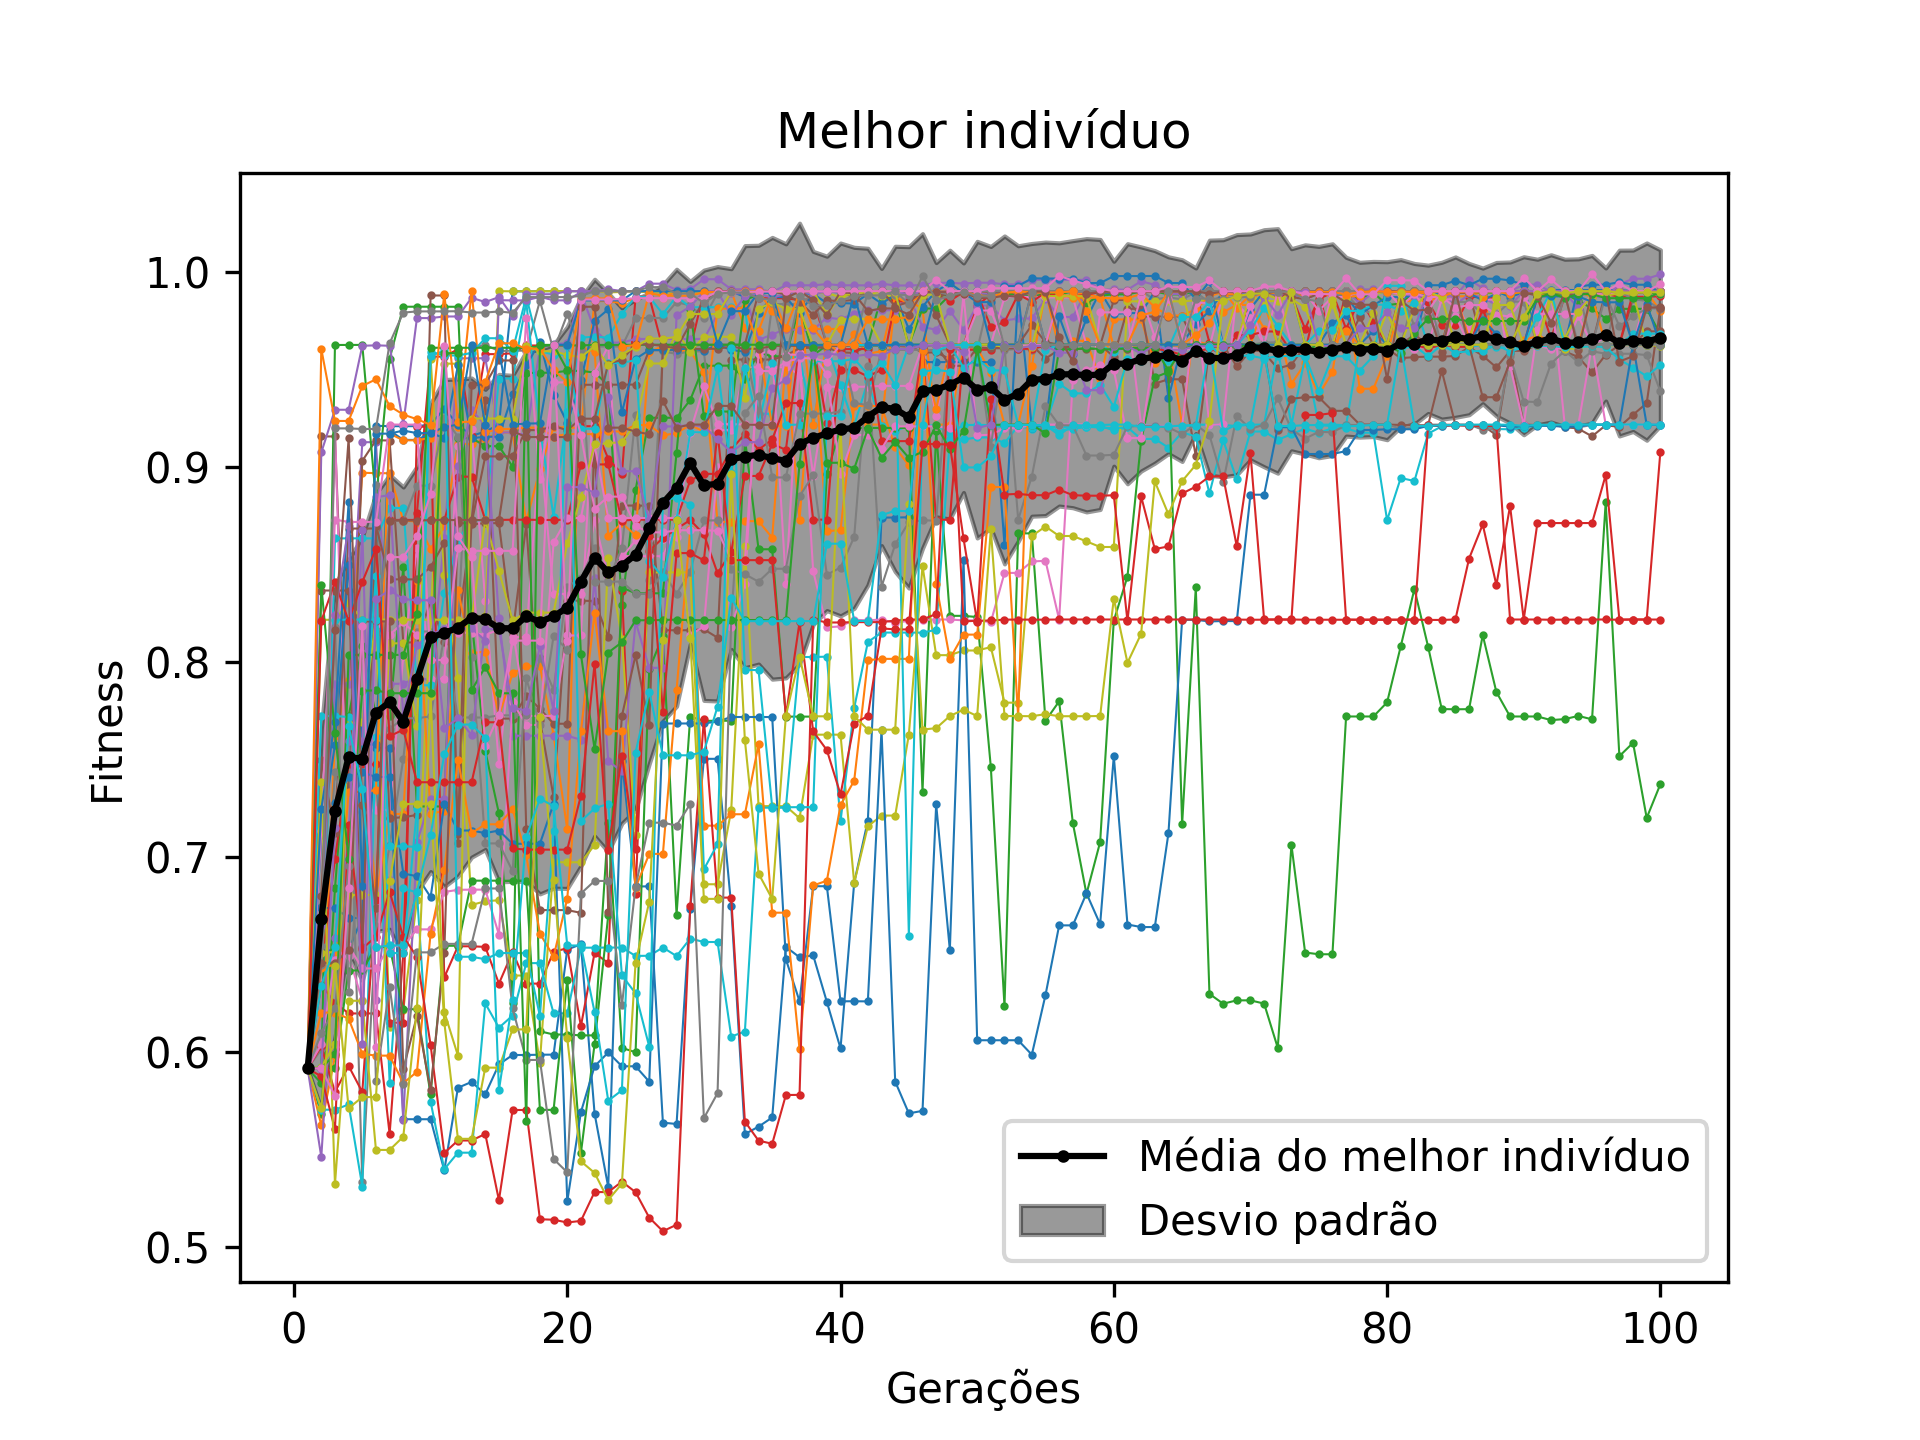
\includegraphics[width=1\textwidth]{sec-02/f6_2p_fitness_vs_gen_best.png}
		\caption{Melhores indíviduos de todos os experimentos ao longo das gerações.
		Em preto é mostrado o comportamento médio dos 50 experimentos. }
	\end{subfigure}
	\hfill
	\begin{subfigure}{.45\textwidth}
		\centering
		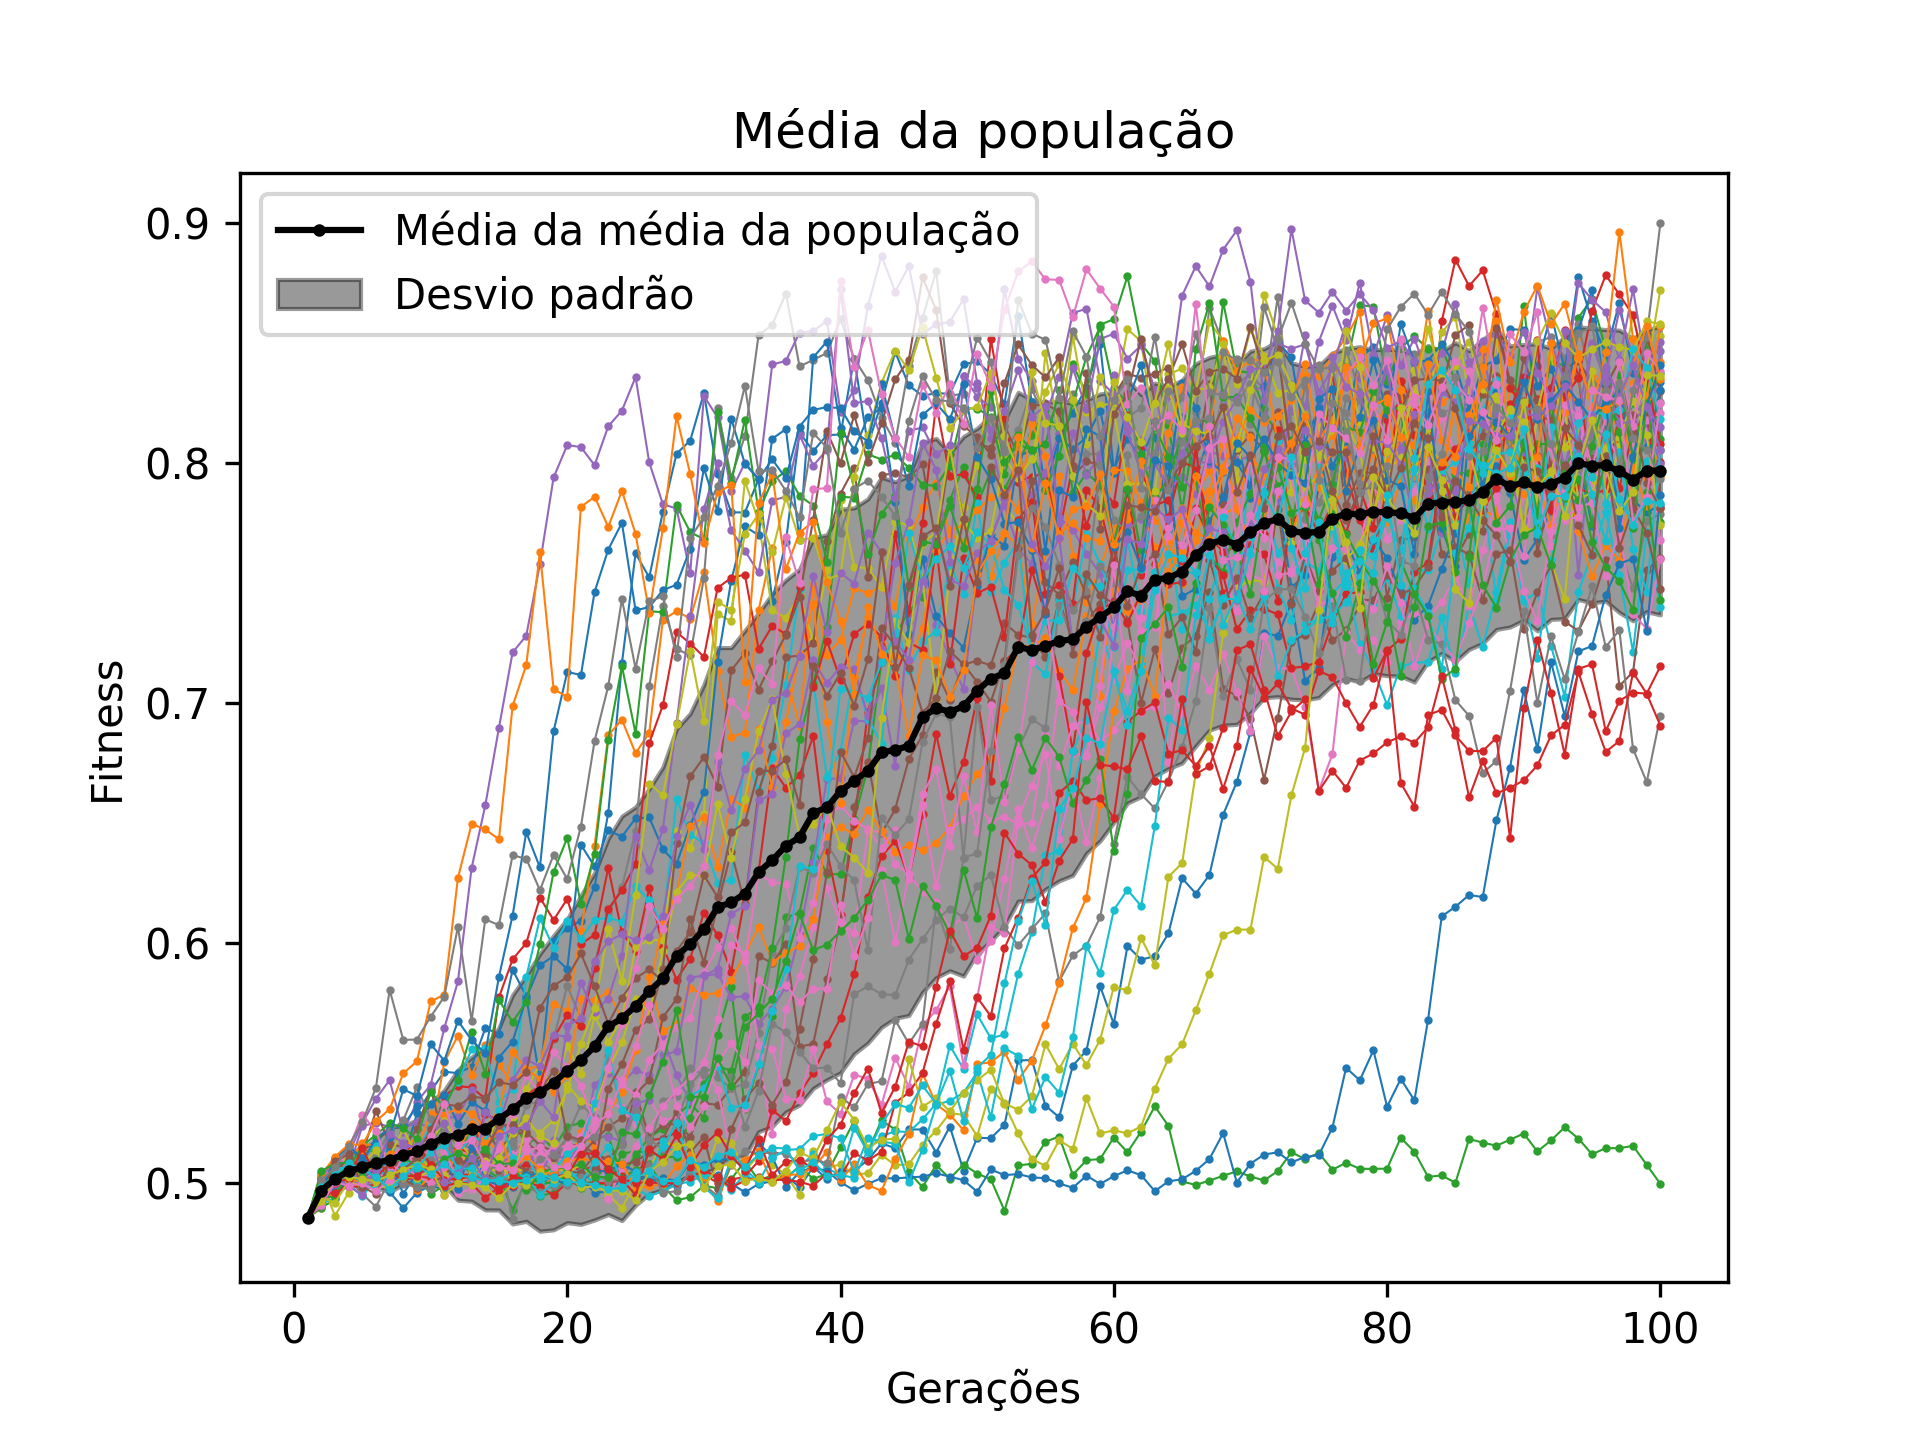
\includegraphics[width=1\textwidth]{sec-02/f6_2p_fitness_vs_gen_pop.png}
		\caption{Média da população de todos os experimentos ao longo das gerações.
		Em preto é mostrado o comportamento médio dos 50 experimentos.}
	\end{subfigure}
	\caption{Resultados obtidos para o caso de cruzamento de 2 pontos apresentado na tabela~\ref{tab:f6_crux}}
\end{figure}


	\begin{figure}[htb]
	\begin{subfigure}{.45\textwidth}
		\centering
		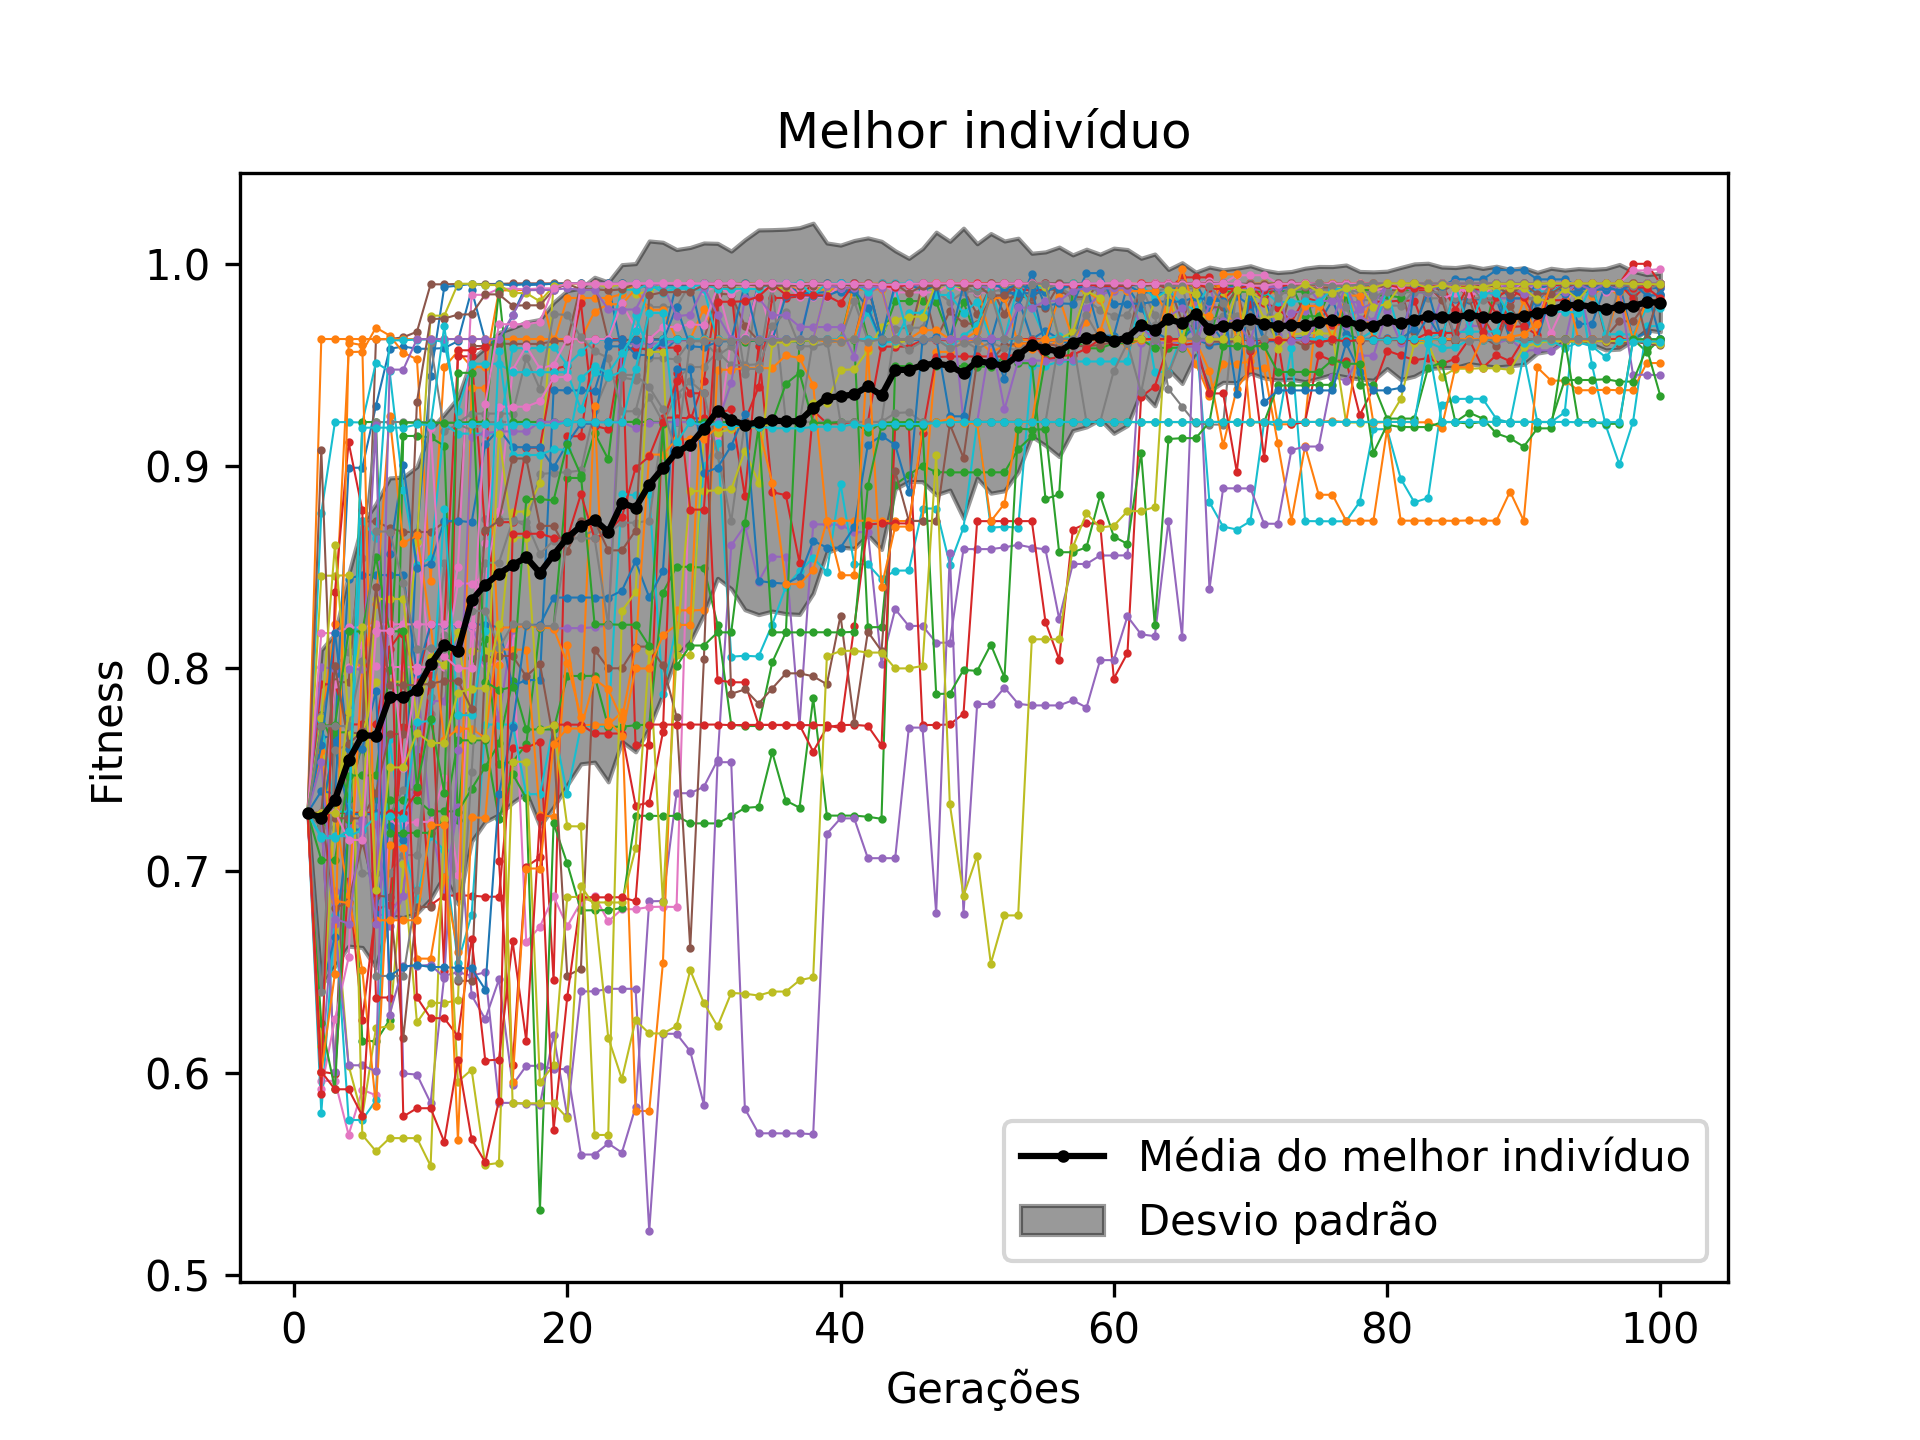
\includegraphics[width=1\textwidth]{sec-02/f6_10p_fitness_vs_gen_best.png}
		\caption{Melhores indíviduos de todos os experimentos ao longo das gerações.
		Em preto é mostrado o comportamento médio dos 50 experimentos. }
	\end{subfigure}
	\hfill
	\begin{subfigure}{.45\textwidth}
		\centering
		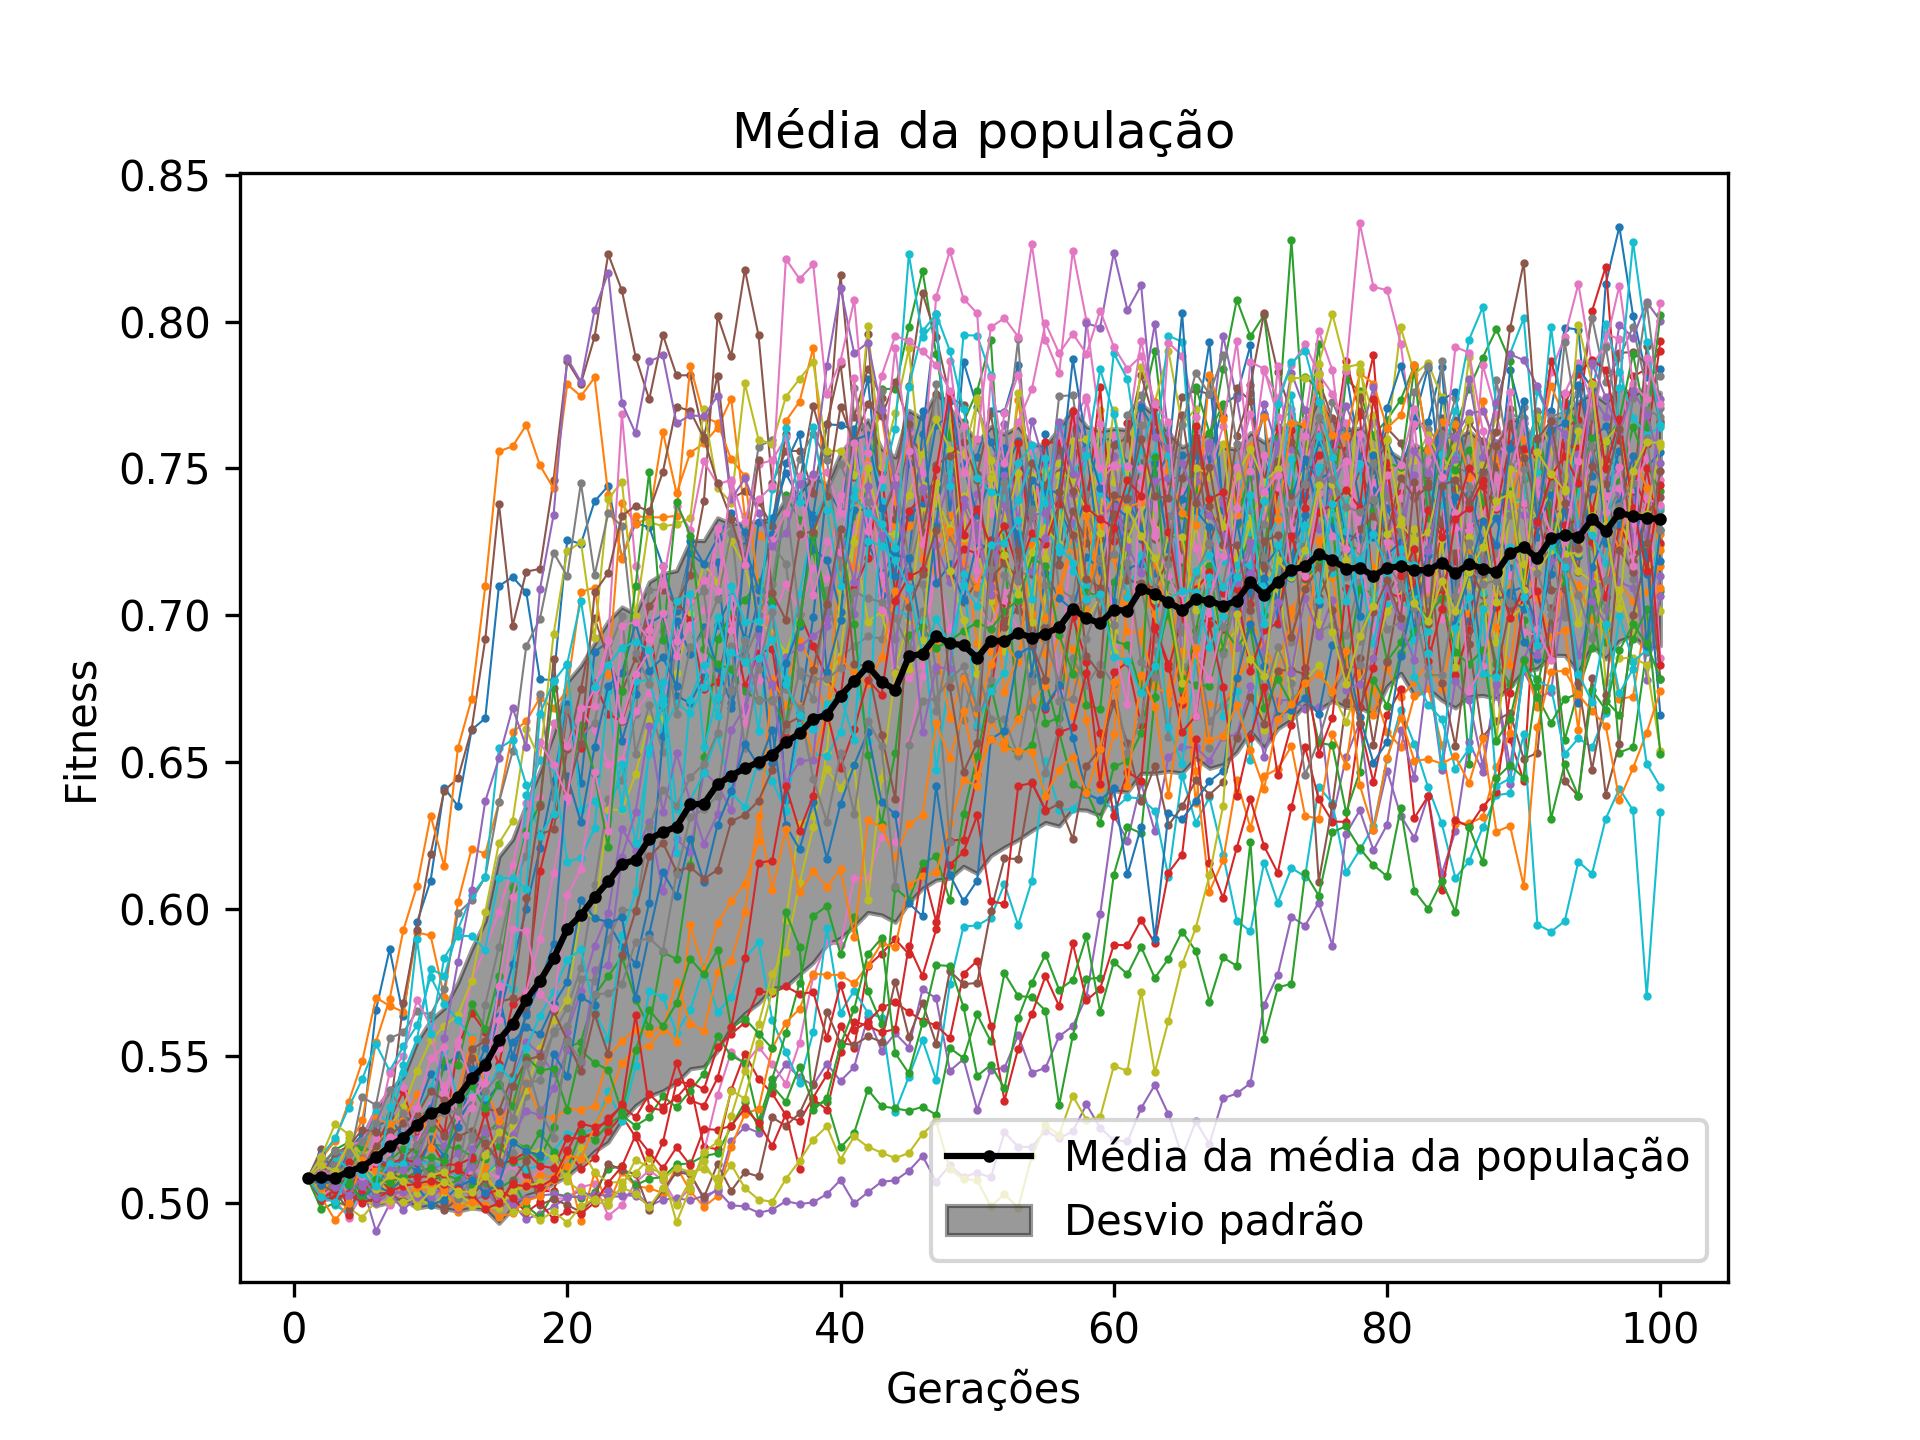
\includegraphics[width=1\textwidth]{sec-02/f6_10p_fitness_vs_gen_pop.png}
		\caption{Média da população de todos os experimentos ao longo das gerações.
		Em preto é mostrado o comportamento médio dos 50 experimentos.}
	\end{subfigure}
	\caption{Resultados obtidos para o caso de cruzamento de 10 pontos apresentado na tabela~\ref{tab:f6_crux}}
\end{figure}


	\begin{figure}[htb]
	\begin{subfigure}{.45\textwidth}
		\centering
		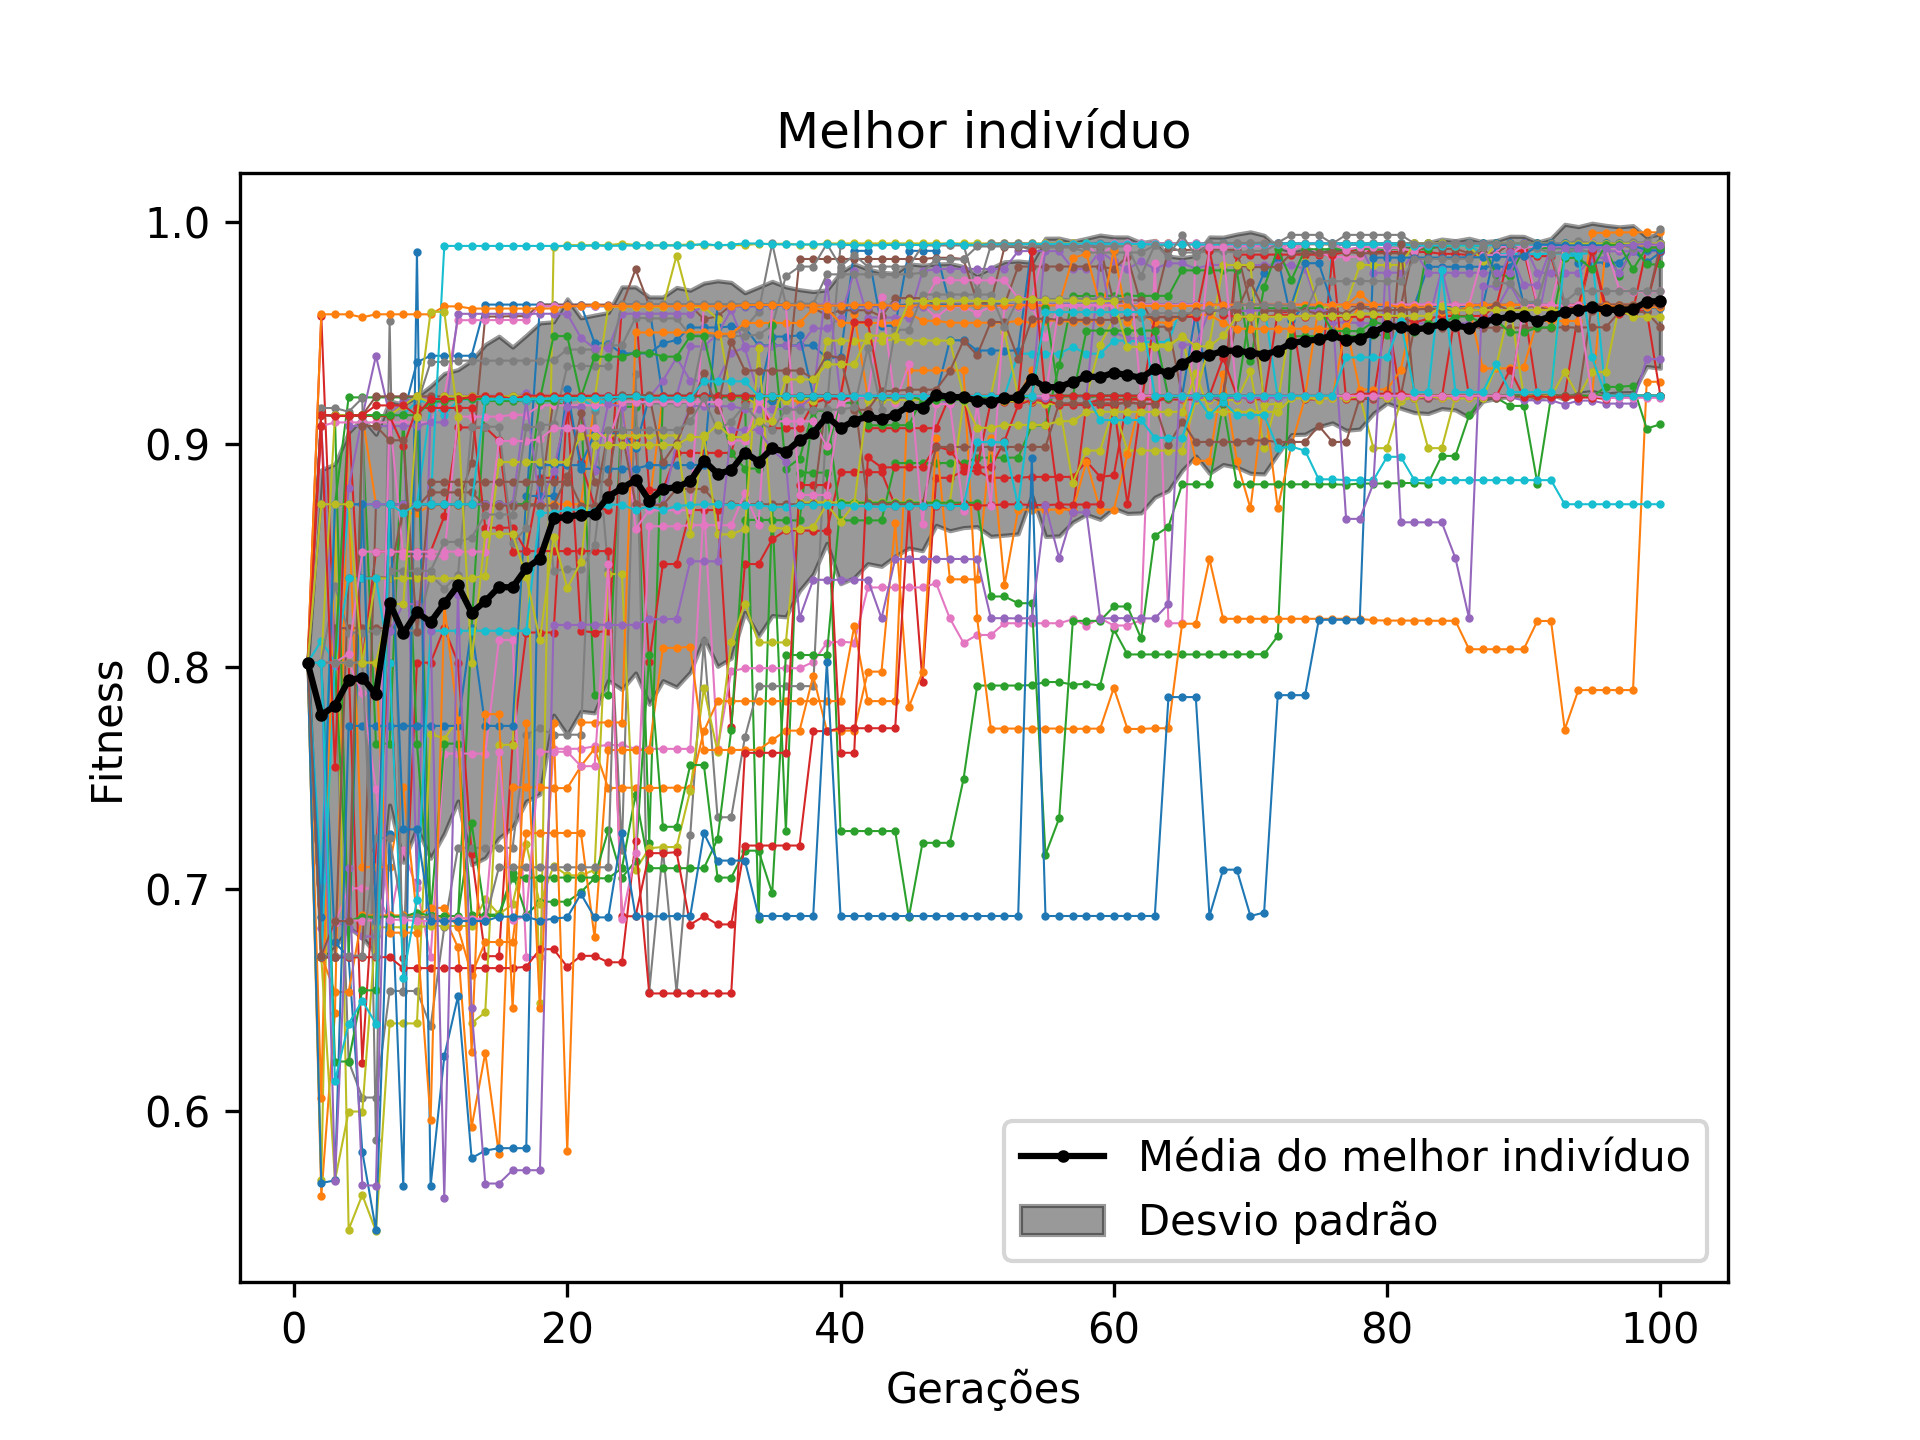
\includegraphics[width=1\textwidth]{sec-02/f6_u_fitness_vs_gen_best.png}
		\caption{Melhores indíviduos de todos os experimentos ao longo das gerações.
		Em preto é mostrado o comportamento médio dos 50 experimentos. }
	\end{subfigure}
	\hfill
	\begin{subfigure}{.45\textwidth}
		\centering
		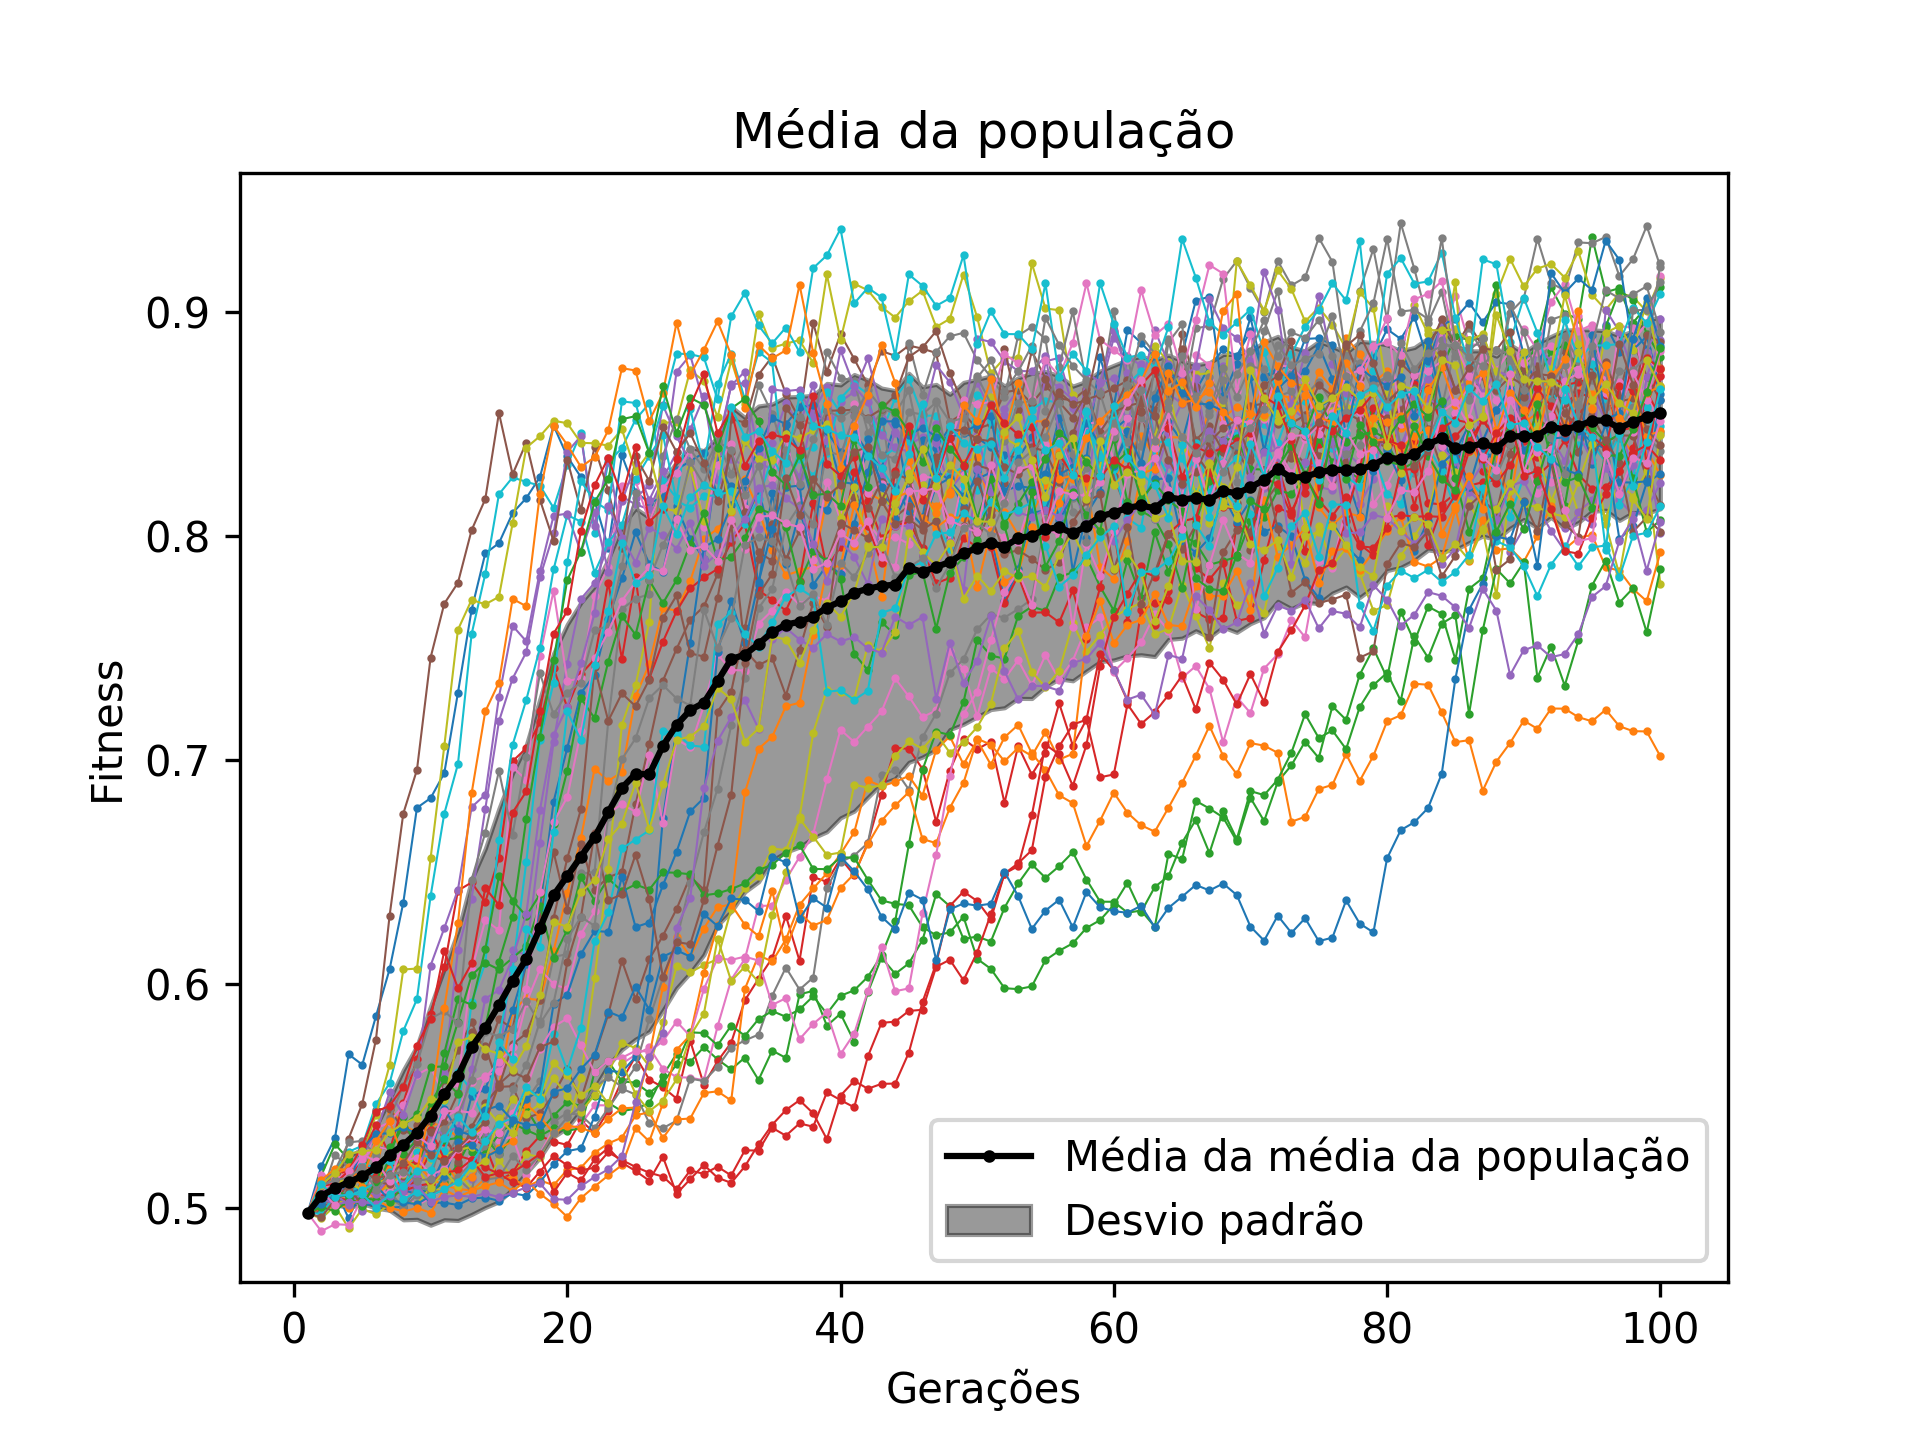
\includegraphics[width=1\textwidth]{sec-02/f6_u_fitness_vs_gen_pop.png}
		\caption{Média da população de todos os experimentos ao longo das gerações.
		Em preto é mostrado o comportamento médio dos 50 experimentos.}
	\end{subfigure}
	\caption{Resultados obtidos para o caso de cruzamento uniforme apresentado na tabela~\ref{tab:f6_crux}}
\end{figure}